\documentclass[a4paper]{scrartcl}
\usepackage[utf8]{inputenc}
\usepackage[english,ngerman]{babel}
\usepackage[autostyle,german=guillemets]{csquotes}
\usepackage{parskip}
\usepackage{scrpage2}
\usepackage{graphicx}
\usepackage{tabularx}
\usepackage{todonotes}
\usepackage[nottoc]{tocbibind}
\usepackage{upquote}
\usepackage{listings}
\usepackage{caption}
\usepackage{courier}
\usepackage{chngcntr}
\usepackage{hyperref}
\hypersetup{
	colorlinks,
	citecolor=black,
	filecolor=black,
	linkcolor=black,
	urlcolor=black
}

%opening
\title{Technische Dokumentation zur erstellten Anwendung,\\
	Modul: Internetanwendungen für mobile Geräte,\\Sommersemester 2015}
\author{Christian Halfmann (CH)\\Andreas Willems (AW)}
\date{\today}

\begin{document}
	% config for listings
	\lstset{
		language=HTML,
		%		extendedchars=true,
		escapeinside={\%*}{*)},
		showstringspaces=false,
		captionpos=b,
		basicstyle=\footnotesize\ttfamily,
		numbers=left,
		numberblanklines=true,
		tabsize=4,
		breaklines=true,
		literate={ä}{{\"a}}1
		{ö}{{\"o}}1
		{ü}{{\"u}}1 
	}
\maketitle

\begin{abstract}
Die erstellte Anwendung ermöglicht das Abrufen von Fotos aus einer Fotosession über ein mobiles Endgerät (z.B. Smartphone) über das Internet. Hierzu wurden ein Web-Client, ein Web-Server sowie ein Datenserver erstellt.
\end{abstract}
%\newpage
%\listoftodos
\tableofcontents
\newpage
\section{Allgemeine Funktionsweise (AW)}
Der Kunde eines Fotografen bekommt nach einer Fotositzung (Session) eine Karte mit 
einer Session-ID überreicht. Anhand dieser ID, welche sich in der aufgerufenen 
Anwendung eingeben lässt, werden die Bilder aus der Session beim Kunden im Endgerät
(Desktop-Browser oder Smartphone-Browser) dargestellt.

Der generelle Aufbau lässt sich der folgenden Abbildung \ref{fig_genereller_aufbau} entnehmen.

\begin{figure}[h]
	\centering
	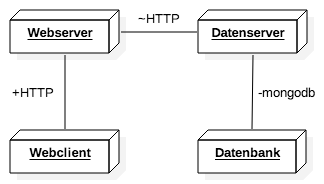
\includegraphics[width=14cm]{bilder/genereller_aufbau}
	\caption{Genereller Aufbau der Anwendung}
	\label{fig_genereller_aufbau}
\end{figure}

Wie in der Grafik zu sehen ist, besteht die Anwendung aus vier den Komponenten
\begin{itemize}
	\item \textbf{Webclient}: diese Komponente ist für den Nutzer sichtbar und dient der Interaktion mit der Anwendung
	\item \textbf{Webserver}: der Webserver nimmt Anfragen des Clients entgegen, beantwortet sie entweder selber oder leitet sie an den Datenserver weiter und gibt Antworten des Datenservers an den Webclient weiter
	\item \textbf{Datenserver}: der Datenserver nimmt Anfragen des Webservers entgegen und dient der Interaktion mit der Datenbank
	\item \textbf{Datenbank}: die Datenbank dient der persistenten Haltung von Sitzungsdaten und Fotos
\end{itemize}

Im Folgenden werden die einzelnen Komponenten weiter vorgestellt und ihre Funktionsweise erläutert.
\clearpage
\section{Webclient (CH)}
\label{section_webclient}
Der Webclient ist die Schnittstelle zwischen Nutzer und Anwendung. Nach Aufruf der Applikation wird der Nutzer aufgefordert seine Session-ID einzugeben. Ist diese gültig, gelangt er in seinen persönlichen Bereich. Dort wird er mit seinem Namen begrüßt und kann die Bilder aus seiner Fotosession betrachten. 

Die einzelnen Bilder werden zunächst zur Übersicht in einer Galerie mit quadratischen Thumbnails angezeigt. Durch Klick auf ein Thumbnail wird das entsprechende Bild vergrößert bzw. das Orginal-Bild angezeigt. Hierbei bietet die Galerie vier verschiedene Ansichtsmöglichkeiten. Auf Smartphones fällt die Auswahlmöglichkeit weg und die Bilder werden initial in der Borderless / Fullscreen Ansicht Dargestellt. 

\begin{itemize}
	\item Lightbox
	\item Borderless
	\item Lightbox / Fullscreen
	\item Borderless / Fullscreen
\end{itemize}

\begin{figure}[h]
	\centering
	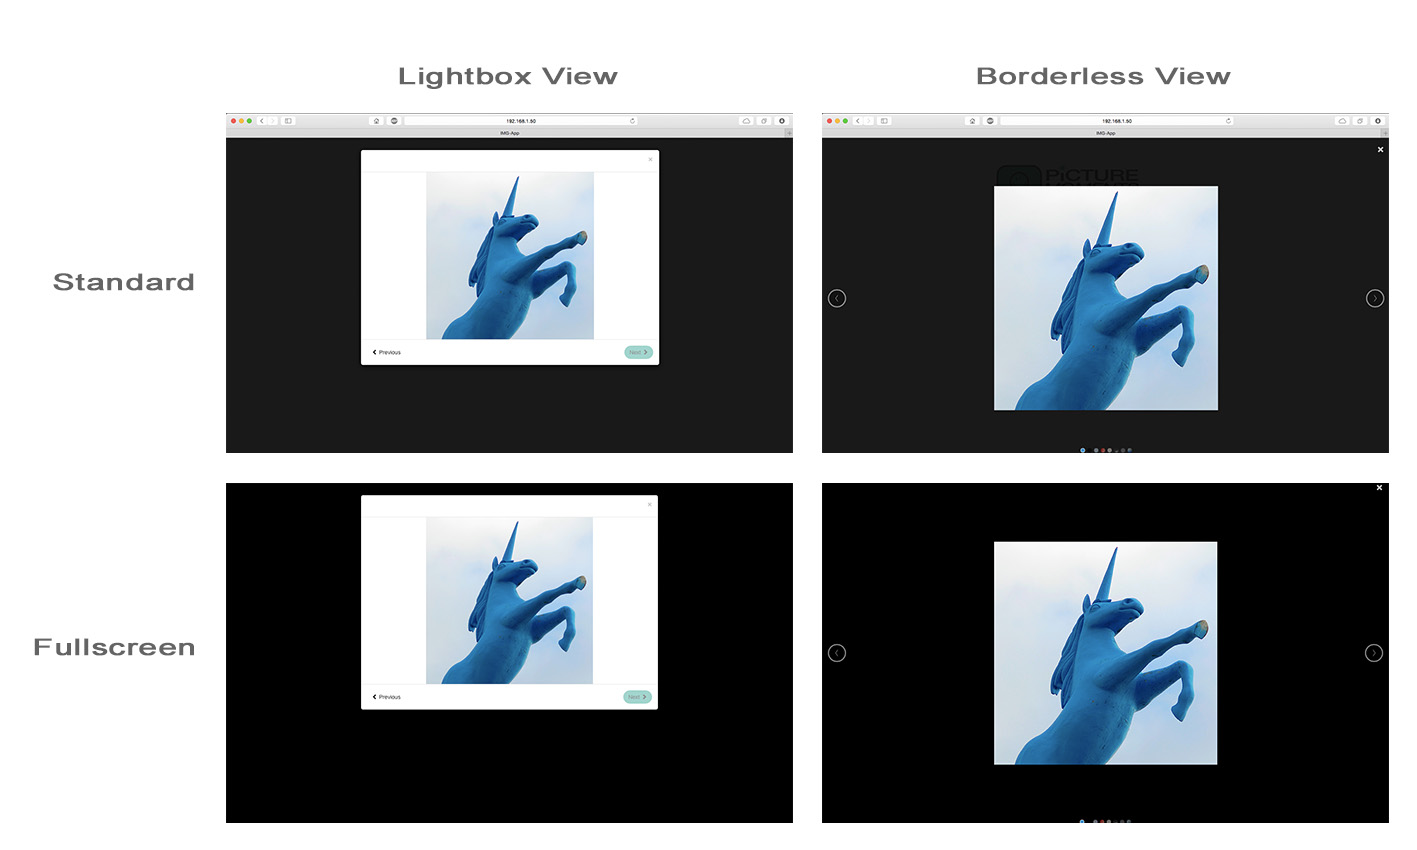
\includegraphics[width=14cm]{bilder/gallery_view}
	\caption{Galerie Ansichten}
	\label{fig_galerie_ansichten}
\end{figure}

In der Galerieansicht lässt sich jeweils zu dem nächsten oder vorherigen Bild via Button oder Pfeiltasten in Desktop Borwsern oder via Touch-Slide auf mobilen Endgeräten navigieren. 

\subsection{Schnittstellen}
Der Webclient hält folgende Schnittstellen bereit:

\begin{table}[h]
	\begin{center}
		\begin{tabularx}{\textwidth}{|c|l|X|}
			\hline
			\textbf{Methode} & \textbf{Pfad} & \textbf{Funktion}\\
			\hline
			GET & / & ruft die Datei index.html auf und bewirkt den Start der Anwendung \\
			\hline
			GET & /api/sessions/:id & ruft die Session mit gegebenen ID auf \\
			\hline
			GET & /api/thumbnails/:id & ruft ein Thumbnail des Bildes mit gegebenen ID ab \\
			\hline
			GET & /api/images/:id & ruft ein Bild mit gegebenen ID ab \\
			\hline
		\end{tabularx}
		\caption{Die zu realisierende Schnittstelle}
		\label{tab_api_routes}
	\end{center}
\end{table}

Mit der Eingabe der URL wird zunächst ein GET Request an den Webserver gestellt, der Webserver gib daraufhin die \textit{index.html} zurück.

Die weitere Kommunikation zwischen Client und Webserver verläuft über die im Webclient integrierte AJAX-Engine. Der Client stellt einen GET Request und bekommt die entsprechende Antwort in Form eines JSON Strings oder als Binärdaten zurück (Siehe dazu auch Abschnitt \ref{webserver_schnittstellen} und Abbildung \ref{fig_webserver_webclient})

\subsection{Realisierung}
Der Webclient basiert auf einer Single-Page Anwendung und wurde mittels der Grundelemente HTML (\textit{index.html}), CSS (\textit{style.css}), JavaScript (\textit{app.js}) implementiert. 

Neben diesen drei Elementen wurde zur Realisierung der Website das Framework Bootstrap und die JavaScript Bibliothek jQuery genutzt. Außerdem wurde zur Erstellung der Galerie auf die Bootstarp Image Gallery blueimp  zurückgegriffen.

Entsprechende Codezeilen des Bootstrap Stylesheets werden durch das Stylesheet \textit{style.css}, was individuelle Designvorgaben enthält, überschrieben. 

Die \textit{index.html} gibt die Struktur der Web-Anwendung vor. Sie beinhaltet das Logo, ein Jumbotron als Textfeld, das Formular zur Eingabe der Session ID und die entsprechenden Button.  Die Darstellung der Seite wird durch die \textit{app.js} gesteuert. Die Elemente werden je nach Bedarf ein- oder ausgeblendet. Dialogtexte sowie die Galerie werden dynamisch erzeugt aus der \textit{app.js} erzeugt. 

Des Weiteren stellt die \textit{app.js} die Funktion requestSession zur AJAX Kommunikation zwischen Webclient und Webserver bereit.

\begin{figure}[h]
	\begin{lstlisting}[caption={Auszug aus app.js (Webclient)}, label=list_client]
	function requestSession(evt) {
		var id = $('#inputSessionId').val();
		if (id !== '') {
		    var jqxhr = $.ajax('/api/sessions/' + id)
		    .done(function() {})
		    .success(function(data, textStatus) {
		        appendSessionView(data);
		    })
		    .fail(function(err) {
		        $('#greeterHeading').css({"color": "#C1121C"}).html(
			        'Die eingegebene Session ID ist nicht vergeben.'  
			        + 'Bitte kontrolliere Deine Eingabe oder versuche ' 
			        + 'es zu einem späteren Zeitpunkt noch einmal.');
			})
			.always(function() {});
		} else {
			$('#greeterHeading').css({"color": "#C1121C"}).html(
			    'Es wurde keine Eingabe getätigt. '
			    + 'Bitte gib Deine Session-ID ein.');
		}
	}
	\end{lstlisting}
\end{figure}

Der Client ruft hierbei Daten vom Webserver, die dort unter einer bestimmten Session ID gespeichert sind, ab. Bei einer ungültigen ID sendet der Webserver den Fehlercode 404 zurück an den Webclient und der Fail-Zweig der If-Abfrage wird ausgeführt. Bei einer gültigen Session ID wird der Success-Zweig ausgeführt und die Daten vom Webserver an die Funktion appendSessionView übergeben.

In der Funktion appendSessionView werden die Daten vom Webserver verarbeitet und dynamisch in die \textit{index.html} übergeben.

\begin{figure}[h]
	\begin{lstlisting}[caption={Auszug aus app.js (Webclient)}, label=list_client]
	var imagesHTML = '';
	sessionData.images.forEach(function(image) {
		var link = '<div class="col-xs-6 col-sm-5 col-md-4 col-lg-3">'
			+ '<a id="thumbnail" href="/api/images/' + image + '" '
			+ 'class="thumbnail" data-gallery>';
		link += '<img src="/api/thumbnails/'
			+ image + '" class="img-responsive" width="" height="" alt="' 
			+ image + '" /></a>';
	
		link += '</div>';
		imagesHTML += link;
	});
	\end{lstlisting}
\end{figure}

Für jedes Bild wird hier in HTML-Syntax eine Div-Box mit den entsprechenden Attributen erstellt. 

\begin{figure}[h]
	\begin{lstlisting}[caption={Auszug aus app.js (Webclient)}, label=list_client]
	var name = sessionData.client.firstname + ' ' 
		+ sessionData.client.lastname;
	$('#greeterHeading')
		.css({"color": "#8D9091"})
		.html('Hallo ' + name 
			+ '!<br/> Die Bilder Deiner Session liegen hier bereit. ' 
			+ 'Du kannst Dich durch alle Bilder durchklicken und '
			+ 'sie online betrachten. Viel Spass!');
	\end{lstlisting}
\end{figure}


Auch der Name wird aus den JSON Daten des Servers hier verarbeitet und mit weiterem Text an die index.html übergeben. 

Die Anwendung soll sowohl für Mobile- als auch für Desktopdevices geeignet sein. Daher soll es einige Unterschiede in der Darstellung das jeweilige Device geben. Beispielweise die eingangs erwähnte Darstellung der Bilder (initiale Ansicht in der Lightbox bei Desktop-Browsern mit der Option diese zu verändern und die Borderless/Fullscreen Ansicht für mobile Endgeräte). 

Die Unterscheidung der Geräte wird durch Funktionen, die die entsprechenden Geräte erkennen und an die Variable isMobile zurück geben. Durch eine If-Abfrage wird die Darstellung der Website für das entsprechende Device angepasst.

\begin{figure}[h]
	\begin{lstlisting}[caption={Auszug aus app.js (Webclient)}, label=list_client]
	// Variable to detect mobile devices
	var isMobile = {
	    Android: function() {
			return navigator.userAgent.match(/Android/i);
		},
		BlackBerry: function() {
			return navigator.userAgent.match(/BlackBerry/i);
		},
		iOS: function() {
			return navigator.userAgent.match(/iPhone|iPad|iPod/i);
		},
		Opera: function() {
			return navigator.userAgent.match(/Opera Mini/i);
		},
		Windows: function() {
			return navigator.userAgent.match(/IEMobile/i);
		},
		any: function() {
			return (isMobile.Android() || isMobile.BlackBerry()
				|| isMobile.iOS() || isMobile.Opera() || isMobile.Windows());
		}
	};
	
	// Gallery view for mobile and desktop devices
	if(isMobile.any()) {
		// Fullscreen and borderless gallery view for mobile devices
		$('#borderless-checkbox').prop('checked', function () {
			var borderless = $(this).is(':checked');
			$('#blueimp-gallery')
				.data('useBootstrapModal', !borderless);
			$('#blueimp-gallery')
				.toggleClass('blueimp-gallery-controls', borderless);
		});
	
		$('#fullscreen-checkbox').prop('checked', function () {
			$('#blueimp-gallery').data('fullScreen', $(this).is(':checked'));
		});
	} else {
		// Initial Lightbox view for desktop devices
		$('#borderless-checkbox').on('change', function () {
			var borderless = $(this).is(':checked');
			$('#blueimp-gallery')
				.data('useBootstrapModal', !borderless);
			$('#blueimp-gallery')
				.toggleClass('blueimp-gallery-controls', borderless);
		});
		$('#fullscreen-checkbox').on('change', function () {
			$('#blueimp-gallery')
				.data('fullScreen', $(this).is(':checked'));
		});
	}
	
	\end{lstlisting}
\end{figure}

In diesem Beispiel wird die Ansichtsart der Bilder für die entsprechenden Devices 
festgelegt. Im ersten If-Zweig, welchher bei der Nutzung mobiler Geräte aufgerufen 
wird, werden durch prop() die Checkboxen, welche zur Auswahl der Darstellung 
dienen, initial als checkt gesetzt und somit die Darstellung auf Borderless/Fullscreen 
gesetzt.
\clearpage
\section{Webserver (AW)}
\label{section_webserver}
Der Webserver nimmt Anfragen des Clients über HTTP entgegen. Er liefert zum einen die 
Internetseite an den Client aus, über die der Benutzer mit der Anwendung interagiert und 
kommuniziert zum anderen mit dem Datenserver.

Der typische Ablauf der Kommunikation zwischen Webclient und Webserver ist in der 
folgenden Abbildung \ref{fig_webserver_webclient} dargestellt:

\begin{figure}[h]
	\centering
	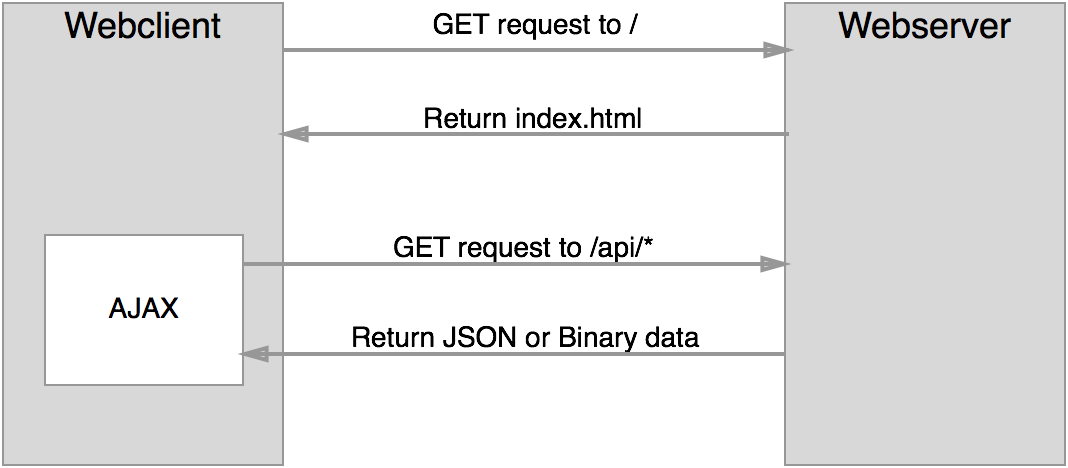
\includegraphics[width=\textwidth]{bilder/abbildung_webserver_webclient}
	\caption{Kommunikation zwischen Webclient und Webserver}
	\label{fig_webserver_webclient}
\end{figure}

Die Abbildung zeigt, wie der Webserver eine Anfrage an 
den Webserver stellt und der mit der Rückgabe der Datei \textit{index.html} antwortet. Da es sich um eine Single-Page-Anwendung handelt, liefert der Webserver nur dieses eine Seite / Page aus.

In der Abbildung \ref{fig_webserver_webclient} ist weiter vereinfacht dargestellt, wie die weitere Kommunikation zwischen Webclient und Webserver über die im Webclient integrierte AJAX\footnote{AJAX (Asynchronous JavaScript and XML): Konzept zur asynchronen Datenübertragung}-Engine ausgeführt wird.
\clearpage
\subsection{Schnittstellen}
Der Webserver hält die in der folgende Tabelle \ref{tab_api_routes} dargestellten Schnittstelle bereit, an die der Webclient 
Anfragen richten kann:
\begin{table}[h]
	\begin{center}
		\begin{tabularx}{\textwidth}{|c|l|X|}
			\hline
			\textbf{Methode} & \textbf{Pfad} & \textbf{Funktion}\\
			\hline
			GET & / & ruft die Datei index.html auf und bewirkt den Start der Anwendung \\
			\hline
			GET & /api/sessions/:id & ruft die Session mit gegebenen ID auf \\
			\hline
			GET & /api/thumbnails/:id & ruft ein Thumbnail des Bildes mit gegebenen ID ab \\
			\hline
			GET & /api/images/:id & ruft ein Bild mit gegebenen ID ab \\
			\hline
		\end{tabularx}
		\caption{Die zu realisierende Schnittstelle}
		\label{tab_api_routes}
	\end{center}
\end{table}

Die in Tabelle angegeben Endpunkte werden wie folgt verwendet:

Der Pfad "/"{} wird durch den Browser des Clients über die Eingabe des Domainnamens aufgerufen.

Der Pfad "/api/sessions/:id"{} wird über einen AJAX-Request aufgerufen, wenn auf der Startseite eine Session-ID 
eingeben wird und der Benutzer den Knopf  "Senden" drückt.

Die Pfade "/api/thumbnails/:id"{} und "/api/images/:id"{} werden in der Datei \textit{index.html} als Attribute des Tags \textit{\textless img\textgreater} verwendet.

\subsection{Realisierung}
Der Webserver ist in JavaScript auf der Node.js-Plattform implementiert. Zur vereinfachten Installation und bequemeren Handhabung von Anfragen an den Server wird das Framework \textit{Express.js} verwendet. 
\clearpage
Die Darstellung der Ordnerstruktur enthält folgende Abbildung \ref{fig_struktur_webserver}:
\begin{figure}[h]
	\centering
	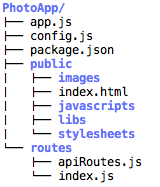
\includegraphics[width=4cm]{bilder/ordnerstruktur_photoapp}
	\caption{Ordnerstruktur des Webservers}
	\label{fig_struktur_webserver}
\end{figure}

Die Datei \textit{package.json} enthält die Konfiguration einer Node.js-Anwendung und 
definiert unter anderem Abhängigkeiten zu Paketen.

Die Datei \textit{config.js} enthält die URL und Ports der beteiligten Server.

In der Datei \textit{app.js} sind die Befehle zur Erzeugung des Web-Servers enthalten. Weiter werden in dieser Datei die übrigen Dateien und die Routen importiert. In Listing \ref{list_server} ist die Datei auszugsweise vorgestellt.

\begin{figure}[h]
\begin{lstlisting}[caption={Auszug aus app.js}, label=list_server]
var express	= require("express"); // import express.js module
var app		= express(); // initialize app / server
var indexRoutes = require("'./routes/index"); // import routes
var apiRoutes = require("./routes/apiRoutes"); // import more routes

app.use("/", routes); // use routes for requests to server
app.listen(60127); // start server listening on port 60127
\end{lstlisting}
\end{figure}

Das Listing zeigt, wie zunächst die verwendeten Module mit \textit{require} importiert werden und die Anwendung anschließend Anwendung initialisiert wird. Im Anschluss werden die importierten Routen in die Anwendung integriert und zum Schluss der Server gestartet. Der Server hört auf Anfragen an den definierten Port.

Die einzelnen Endpunkte der Schnittstelle (Routen) sind wie in Listing \ref{list_api} abgebildet implementiert:

\begin{figure}
\begin{lstlisting}[caption={Auszug aus den Dateien routes/index.js und routes/apiRoutes.js}, label=list_api]
/* GET home page. */
router.get("/", function(req, res, next) {
    res.sendFile('index.html');
});

/* GET requests to /api/sessions/:id, /api/thumbnails/:id, /api/images/:id */
router.get("/sessions/:id", function(req, res, next) {
    var sessionId = req.params.id;
    // create options object for the following request
	var options = {
		host: serverData.host,
		port: serverData.port,
		path: "/api/sessions/" + sessionId,
		method: "GET",
		accept: "application/json"
	};

	// create and send request
	http.request(options, function(response) {
	// check response for error
	    if (response.statusCode == "404") {
	        return res.status(404).send();
		}
		// in case of images pipe incoming stream to outgoing stream
		// response.pipe(res);
		
		var resData = "";
		// react to the server's response...
		response.on("data", function(data) {
		// ... by passing the responded data to variable resData...
		    resData += data;
		});
		
		// ...and returning it to the client in the end
		response.on("end", function() {
		    // ...as JSON if dealing with session data...
		    res.json(JSON.parse(resData));
		    // ...or as binary data in case of images
		    // res.set("Content-Type", contentType);
		    // res.end(resData, "binary");
		});
	}).end();
});
\end{lstlisting}
\end{figure}

Die erste Route in den Zeilen 2-4 reagiert auf die Anfrage an den Pfad "/".
Sie sendet daraufhin die HTML-Datei an den Client zurück.

Die zweite Route in den Zeilen 7 bis 40 ist verantwortlich für Anfragen an den Pfad 
"/api/sessions/:id", die Funktionsweise ist jedoch identisch zur Anfragen 
an "/api/images/:id"{} und "/api/thumbnails/:id".

Wenn eine Anfrage an diese Pfade eingeht, wird eine entsprechende HTTP-Anfrage 
an den Datenserver gerichtet und die zurückerhaltene Antwort an den Webclient 
weitergeleitet.

Zunächst wird aus den Request-Parametern die ID ausgelesen (Zeile 8). Anschließend 
wird ein Objekt erzeugt, das die Art der ausgehenden HTTP steuert (Zeilen 10-16).
Der HTTP Request wird mit den gegebenen Optionen an den Datenserver gesandt (Zeile 19 bis 42).
Die zurückkommende Antwort wird verarbeitet und an den Webclient weitergeleitet (Zeilen 21 bis 40).

Die Anwendung enthält im Übrigen den Ordner \textit{public}, der die Dateien des Webclients 
enthält (vgl. Abschnitt \ref{section_webclient}).



\section{Datenserver}
Der Datenserver nimmt über eine Schnittstelle im REST-Design\footnote{REST 
(Representational State Transfer): Programmierparadigma, um Ressourcen im Web über 
definierte und eindeutige Schnittstellen zu erreichen} Anfragen über HTTP\footnote{HTTP 
(Hyper Text Transfer Prototcol)} entgegen und wandelt diese in Datenbankanfragen um. 
Nach erfolgter Antwort gibt der Datenserver die Daten aus der Datenbank an den Client 
über HTTP zurück.
\section{Datenbank}



\end{document}
